% 原书第3章 PDF 页49—62，3.3，印刷页221—234。
\section{函数值性状的基因—基因交互作用分析}
\subsection{引言}

许多生理性状虽然以函数形式测量，但目前广泛用于人体函数值性状交互作用分析的方法，仍与传统单值数量性状的方法相同，即把一个数值作为数量性状。这些方法用汇总统计量度量或表示函数值性状。因此，前面各章为标量数量性状交互作用分析开发的全部方法，都可用于函数值性状的交互作用分析。函数值性状的数量遗传分析，有助于理解性状整个动态过程的遗传控制，并提高检出上位性的统计功效。尽管数量性状的遗传研究已广泛应用，技术也有长足发展，函数值性状的数量遗传分析相对仍不充分。

快速且成本较低的下一代测序（NGS）技术，将产生规模空前、维数极高的遗传变异数据，使几乎完整地评价常见变异与罕见变异成为可能，为全面编目人类遗传变异提供了有力工具。然而，利用 NGS 数据分析交互作用仍面临关键障碍：多数传统统计方法采用基于 SNP 的两两上位性检验，最初是为检验常见变异的交互作用设计的。这些方法难以应用于罕见变异，因为其第一类错误率高、计算时间难以承受、多重检验带来的统计挑战严重，而且检出罕见变异之间交互作用的功效低。

为弥补这一不足，本节介绍基于响应与预测变量均为函数型的非线性函数型回归模型的新方法，用于函数值性状的上位性分析。这类方法能够同时捕捉性状和基因组区域中隐含的全部时间与空间信息，同时大幅降低维数。函数值—函数型回归（functional valued-functional regression，F-FRG）模型，对两个基因组区域（或基因）内全部可能 SNP 配对之间的交互作用作联合检验。

如第7.5节所述，典型相关分析（CCA）及函数型典型相关分析可作为检验基因—基因和基因—环境交互作用的统一框架。最后还将简要讨论如何用函数型 CCA 分析函数值性状的交互作用。

\subsection{函数型回归模型}

考虑第 $i$ 个个体随时间变化的性状 $y_i(\tau)$，$\tau\in T_\tau=[0,T_\tau]$，以及两个基因组区域（或基因）$[a_1,b_1]$ 和 $[a_2,b_2]$。设 $x_i(t)$ 和 $x_i(s)$ 分别为第 $i$ 个个体在区域 $[a_1,b_1]$ 和 $[a_2,b_2]$ 上定义的基因型函数。$t$ 和 $s$ 分别是第一、第二个基因组区域中的基因组位置。基因型函数 $x_i(t)$ 和 $x_i(s)$ 定义为
\[
X_i(t)=\begin{cases}
2P_m(t),&\mathrm{MM},\\
P_m(t)-P_M(t),&\mathrm{Mm},\\
-2P_M(t),&\mathrm{mm},
\end{cases}
\qquad
X_i(s)=\begin{cases}
2P_m(s),&\mathrm{MM},\\
P_m(s)-P_M(s),&\mathrm{Mm},\\
-2P_M(s),&\mathrm{mm},
\end{cases}
\]
其中 $M$ 和 $m$ 是基因组位置 $t$ 或 $s$ 处标记的两个等位基因；$P_M(t)$、$P_m(t)$ 及 $P_M(s)$、$P_m(s)$ 分别为位置 $t$ 和 $s$ 处等位基因 $M$ 与 $m$ 的频率。考虑函数型回归模型
\begin{equation}
\begin{aligned}
Y_i(\tau)={}&\mu(\tau)+W_i^T\omega(\tau)
+\int_Tx_i(t)\alpha(t,\tau)\,dt
+\int_Sz_i(s)\beta(s,\tau)\,ds\\
&+\int_T\int_Sx_i(t)z_i(s)\gamma(t,s,\tau)\,ds\,dt+\varepsilon_i(\tau),
\end{aligned}
\tag{3.86}
\end{equation}
其中 $\mu(\tau)$ 是时间 $\tau$ 的总体均值函数，$W_i$ 为第 $i$ 个个体的协变量向量，$\omega(\tau)$ 为协变量相应的效应向量；$\alpha(t,\tau)$ 是第一个基因在基因组位置 $t$、时间 $\tau$ 的遗传加性效应函数；$\beta(s,\tau)$ 是第二个基因在基因组位置 $s$、时间 $\tau$ 的遗传加性效应函数；$\gamma(t,s,\tau)$ 是时间 $\tau$ 处，位于基因组位置 $t$ 和 $s$ 的两个假定数量性状位点（QTL）之间的交互作用效应函数；$\varepsilon_i(\tau)$ 为第 $i$ 个个体在时间 $\tau$ 的未解释效应的残差函数。交互作用函数通过两个基因中基因型函数的二重积分度量。

\subsection{交互作用效应函数的估计}

假设表型函数与基因型函数均已中心化。将基因型函数 $x_i(t)$ 和 $x_i(s)$ 按正交归一基函数展开为
\begin{equation}
x_i(t)=\sum_{j=1}^{\infty}\xi_{ij}\phi_j(t),\qquad
x_i(s)=\sum_{l=1}^{\infty}\eta_{il}\psi_l(s),
\tag{3.87}
\end{equation}
其中 $\phi_j(t)$ 和 $\psi_l(s)$ 是正交归一基函数序列。展开系数 $\xi_{ij}$ 和 $\eta_{il}$ 由下式估计：
\begin{equation}
\xi_{ij}=\int_Tx_i(t)\phi_j(t)\,dt,\qquad
\eta_{il}=\int_Sx_i(s)\psi_l(s)\,ds.
\tag{3.88}
\end{equation}
实际计算中，采用数值积分方法求得展开系数。

将式 (3.87) 代入式 (3.86)，得到
\begingroup
\small
\begin{equation}
\begin{aligned}
Y_i(\tau)={}&\mu(\tau)+W_i^T\omega(\tau)
+\int_T\sum_{j=1}^{J}\xi_{ij}\phi_j(t)\alpha(t,\tau)\,dt
+\int_S\sum_{l=1}^{L}\eta_{il}\psi_l(s)\beta(s,\tau)\,ds\\
&+\int_T\int_S\sum_{j=1}^{J}\xi_{ij}\phi_j(t)
\sum_{l=1}^{L}\eta_{il}\psi_l(s)\gamma(t,s,\tau)\,ds\,dt
+\varepsilon_i(\tau)\\
={}&\mu(\tau)+W_i^T\omega(\tau)
+\sum_{j=1}^{J}\xi_{ij}\int_T\phi_j(t)\alpha(t,\tau)\,dt
+\sum_{l=1}^{L}\eta_{il}\int_S\psi_l(s)\beta(s,\tau)\,ds\\
&+\sum_{j=1}^{J}\sum_{l=1}^{L}\xi_{ij}\eta_{il}
\int_T\int_S\phi_j(t)\psi_l(s)\gamma(t,s,\tau)\,ds\,dt
+\varepsilon_i(\tau)\\
={}&\mu(\tau)+W_i^T\omega(\tau)
+\sum_{j=1}^{J}\xi_{ij}\alpha_j(\tau)+\sum_{l=1}^{L}\eta_{il}\beta_l(\tau)\\
&+\sum_{j=1}^{J}\sum_{l=1}^{L}\xi_{ij}\eta_{il}\gamma_{jl}(\tau)+\varepsilon_i(\tau),
\end{aligned}
\tag{3.89}
\end{equation}
\endgroup
其中
\[
\begin{aligned}
\alpha_j(\tau)&=\int_T\alpha(t,\tau)\phi_j(t)\,dt,\\
\beta_l(\tau)&=\int\beta(s,\tau)\psi_l(s)\,ds,\\
\gamma_{jl}(\tau)&=\int_T\int_S\gamma(t,s,\tau)\phi_j(t)\psi_l(s)\,dt\,ds.
\end{aligned}
\]
参数 $\alpha_j(\tau)$、$\beta_l(\tau)$ 和 $\gamma_{jl}(\tau)$ 称为遗传加性效应及加性 $\times$ 加性效应得分函数。这些得分函数，也可视为遗传效应函数相对于正交归一基函数的展开系数：
\[
\begin{aligned}
\alpha(t,\tau)&=\sum_j\alpha_j(\tau)\phi_j(t),\\
\beta(s,\tau)&=\sum_l\beta_l(\tau)\psi_l(s),\\
\gamma(s,t)&=\sum_j\sum_l\gamma_{jl}(\tau)\phi_j(s)\psi_l(t).
\end{aligned}
\]
令
\[
Y(\tau)=\begin{bmatrix}Y_1(\tau)\\\vdots\\Y_n(\tau)\end{bmatrix},\qquad
e=\begin{bmatrix}1\\\vdots\\n\end{bmatrix},\qquad
W=\begin{bmatrix}W_{11}&\cdots&W_{1d}\\\vdots&\ddots&\vdots\\W_{n1}&\cdots&W_{nd}\end{bmatrix},
\]
\[
\omega(\tau)=\begin{bmatrix}\omega_1(\tau)\\\vdots\\\omega_d(\tau)\end{bmatrix},\qquad
\xi=\begin{bmatrix}\xi_{11}&\cdots&\xi_{1J}\\\vdots&\ddots&\vdots\\\xi_{n1}&\cdots&\xi_{nJ}\end{bmatrix},\qquad
\eta=\begin{bmatrix}\eta_{11}&\cdots&\eta_{1L}\\\vdots&\ddots&\vdots\\\eta_{n1}&\cdots&\eta_{nL}\end{bmatrix},
\]
\[
\xi_i=\begin{bmatrix}\xi_{i1}\\\vdots\\\xi_{iJ}\end{bmatrix},\qquad
\eta_i=\begin{bmatrix}\eta_{i1}\\\vdots\\\eta_{iL}\end{bmatrix},\qquad
\alpha(\tau)=\begin{bmatrix}\alpha_1(\tau)\\\vdots\\\alpha_J(\tau)\end{bmatrix},
\]
\[
\begin{aligned}
\Gamma&=\begin{bmatrix}\xi_1^T\otimes\eta_1^T\\\vdots\\\xi_n^T\otimes\eta_n^T\end{bmatrix}\\
&=\begin{bmatrix}
\xi_{11}\eta_{11}&\cdots&\xi_{11}\eta_{1L}&\cdots&\xi_{1J}\eta_{11}&\cdots&\xi_{1J}\eta_{1L}\\
\cdots&\cdots&\cdots&\cdots&\cdots&\cdots&\cdots\\
\xi_{n1}\eta_{n1}&\cdots&\xi_{n1}\eta_{nL}&\cdots&\xi_{nJ}\eta_{n1}&\cdots&\xi_{nJ}\eta_{nL}
\end{bmatrix},
\end{aligned}
\]
以及
\[
\beta(\tau)=\begin{bmatrix}\beta_1(\tau)\\\vdots\\\beta_L(\tau)\end{bmatrix},\qquad
\varepsilon(\tau)=\begin{bmatrix}\varepsilon_1(\tau)\\\vdots\\\varepsilon_n(\tau)\end{bmatrix}.
\]
式 (3.89) 可写为矩阵形式：
\begin{equation}
Y(\tau)=e\mu(\tau)+W\omega(\tau)+\xi\alpha(\tau)+\eta\beta(\tau)
+\Gamma\gamma(\tau)+\varepsilon(\tau).
\tag{3.90}
\end{equation}
将 $Y(\tau)$、$\mu(\tau)$、$\omega(\tau)$、$\alpha(\tau)$、$\beta(\tau)$、$\gamma(\tau)$ 和 $\varepsilon(\tau)$ 按正交基函数展开，并把展开式代入式 (3.90)，得
\[
\begin{aligned}
Y_i(\tau)&=\sum_{k=1}^{K}y_{ik}\theta_k(\tau),&
\mu(\tau)&=\sum_{k=1}^{K}\mu_k\theta_k(\tau),\\
\omega_j(\tau)&=\sum_{k=1}^{K}\omega_{jk}\theta_k(\tau),&
\alpha_j(\tau)&=\sum_{k=1}^{K}\alpha_{jk}\theta_k(\tau),\\
\beta_j(\tau)&=\sum_{k=1}^{K}\beta_{jk}\theta_k(\tau),&
\gamma_{jl}(\tau)&=\sum_{k=1}^{K}\gamma_{jlk}\theta_k(\tau),\\
\varepsilon_i(\tau)&=\sum_{k=1}^{K}\varepsilon_{ik}\theta_k(\tau).
\end{aligned}
\]
定义展开系数向量与矩阵如下：
\[
Y=\begin{bmatrix}y_{11}&\cdots&y_{1K}\\\vdots&\ddots&\vdots\\y_{n1}&\cdots&y_{nK}\end{bmatrix},\quad
\mu=\begin{bmatrix}\mu_1\\\vdots\\\mu_K\end{bmatrix},\quad
E=\begin{bmatrix}1&\cdots&1\\\vdots&\ddots&\vdots\\1&\cdots&1\end{bmatrix},
\]
\[
\omega=\begin{bmatrix}\omega_{11}&\cdots&\omega_{1K}\\\vdots&\ddots&\vdots\\\omega_{d1}&\cdots&\omega_{dK}\end{bmatrix},\qquad
\alpha=\begin{bmatrix}\alpha_{11}&\cdots&\alpha_{1K}\\\vdots&\ddots&\vdots\\\alpha_{J1}&\cdots&\alpha_{JK}\end{bmatrix},
\]
\[
\beta=\begin{bmatrix}\beta_{11}&\cdots&\beta_{1K}\\\vdots&\ddots&\vdots\\\beta_{L1}&\cdots&\beta_{LK}\end{bmatrix},\qquad
\gamma=\begin{bmatrix}\gamma_{111}&\cdots&\gamma_{11K}\\\vdots&\ddots&\vdots\\\gamma_{JL1}&\cdots&\gamma_{JLK}\end{bmatrix},
\]
以及
\[
\varepsilon=\begin{bmatrix}\varepsilon_{11}&\cdots&\varepsilon_{1K}\\\vdots&\ddots&\vdots\\\varepsilon_{n1}&\cdots&\varepsilon_{nK}\end{bmatrix}.
\]
于是，式 (3.90) 可转换为
\begin{equation}
Y\theta(\tau)=\mu\theta(\tau)+W\omega\theta(\tau)+\xi\alpha\theta(\tau)
+\eta\beta\theta(\tau)+\Gamma\gamma\theta(\tau)+\varepsilon\theta(\tau).
\tag{3.91}
\end{equation}
由于式 (3.91) 对每个时间点 $\tau$ 都成立，两边的系数应当相等。因此，函数型回归模型 (3.91) 进一步转换为标准多元多重回归：
\begin{equation}
Y=E\mu+W\omega+\xi\alpha+\eta\beta+\Gamma\gamma+\varepsilon.
\tag{3.92}
\end{equation}
令
\[
A=[E\ W\ \xi\ \eta\ \Gamma],\qquad
b=\begin{bmatrix}\mu\\\omega\\\alpha\\\beta\\\gamma\end{bmatrix}.
\]
式 (3.92) 可重写为
\begin{equation}
Y=Ab+\varepsilon.
\tag{3.93}
\end{equation}
类似于式 (3.56)，真实值 $Y$ 与预测值 $A\hat b$ 之间的误差平方和定义为
\[
F=\Tr\bigl((Y-Ab)^T(Y-Ab)\bigr)=\Tr(\varepsilon^T\varepsilon).
\]
令 $\partial F/\partial b=-A^T(Y-Ab)=0$，得到参数向量 $b$ 的最小二乘估计：
\begin{equation}
\hat b=(A^TA)^{-1}A^TY.
\tag{3.94}
\end{equation}
协方差矩阵 $\Sigma$ 估计为
\[
\hat\Sigma=\frac{(Y-A\hat b)^T(Y-A\hat b)}{(n-(J+L+JL))k}.
\]

\subsection{检验统计量}

数量性状遗传交互作用研究的核心问题，是检验两个基因组区域（或基因）之间的交互作用。形式上，考虑检验
\[
\gamma(t,s,\tau)=0,\quad \forall t\in[a_1,b_1],\ s\in[a_2,b_2],\ \tau\ni[0,T_\tau],
\]
它等价于检验原假设
\begin{equation}
H_0:\gamma=0.
\tag{3.95}
\end{equation}
以 $\vecop$ 表示向量化运算。为构造检验统计量，首先计算 $\vecop(\hat b)$ 的协方差矩阵。假设
\begin{equation}
\Var\bigl(\vecop(\varepsilon)\bigr)=\Sigma\otimes I_n.
\tag{3.96}
\end{equation}
回顾
\[
\vecop(\hat b)=\bigl[I_n\otimes(A^TA)^{-1}A^T\bigr]\vecop(Y).
\]
因此有
\begin{equation}
\begin{aligned}
\Var\bigl(\vecop(\hat b)\bigr)
&=\bigl[I_K\otimes(A^TA)^{-1}A^T\bigr](\Sigma\otimes I_n)
\bigl[I_K\otimes A(A^TA)^{-1}\bigr]\\
&=\Sigma\otimes(A^TA)^{-1}.
\end{aligned}
\tag{3.97}
\end{equation}
设 $\Lambda$ 为协方差矩阵 $\Var(\vecop(\hat b))$ 的最后 $JLK$ 列和最后 $JLK$ 行构成的矩阵；$\hat\gamma$ 为交互作用估计量，由参数矩阵估计量 $\hat b$ 的最后 $JL$ 行提取得到。检验两个基因组区域 $[a_1,b_1]$ 和 $[a_2,b_2]$ 之间交互作用的统计量定义为
\begin{equation}
T_I=(\vecop(\hat\gamma)^T\Lambda^{-1}\vecop(\hat\gamma).
\tag{3.98}
\end{equation}
在原假设 $H_0:\gamma=0$ 下，$T_1$ 渐近服从自由度为 $JLK$ 的中心 $\chi^2_{(JLK)}$ 分布。

\subsection{模拟研究}
\subsubsection{第一类错误率}

为考察检验统计量的零分布，进行一系列模拟，比较经验水平与名义水平。在三个模型下计算第一类错误率。首先假设具有边际效应的模型：

\textbf{模型1（无边际效应）：}
\[
Y_i(\tau_l)=\mu+\varepsilon_i(\tau_l),\quad l=1,\ldots,L,
\]
其中误差 $\varepsilon_i(t_l)$ 由标准布朗运动生成，时间点 $t_l$ 在区间 $[0,1]$ 上等距分布，考虑 $L=203,040$。

接着考虑一个基因具有边际遗传效应的模型：

\textbf{模型2（第一个基因具有边际效应）：}
\[
Y_i(\tau_l)=\mu+\sum_{j=1}^{J}x_{ij}\alpha_j(\tau_l)+\varepsilon_i(\tau_l),
\]
其中 $x_{ij}$ 是第 $i$ 个个体在第一个基因中第 $j$ 个 SNP 的基因型指示变量；假设遗传加性效应函数为
\[
\alpha_j(\tau_l)=\alpha_j\alpha(\tau_l),\qquad
\alpha_j=(1-P_j)(r_1-1)f_0,\qquad
\alpha(\tau_l)=0.05e^{0.05\tau_l}.
\]
$P_j$ 为第一个基因第 $j$ 个基因组位置处次要等位基因的频率；$\gamma_1=1.01$ 为第一个基因的风险参数；$f_0=1$ 为基线外显率。同样，误差 $\varepsilon_i(t_l)$ 由标准布朗运动生成，时间点 $t_l$ 在区间 $[0,1]$ 上等距分布，考虑 $L=20,30,40$。

\textbf{模型3（两个基因均具有边际效应）：}
\[
Y_i(\tau_l)=\mu+\sum_{j=1}^{J}x_{ij}\alpha_j(\tau_l)
+\sum_{k=1}^{K}z_{ik}\beta_k(\tau_l)+\varepsilon_i(\tau_l),
\]
其中 $z_{ik}$ 是第 $i$ 个个体在第二个基因中第 $k$ 个 SNP 的基因型指示变量。假设遗传加性效应函数为
\[
\beta_k(\tau_l)=\beta_k\beta(\tau_l),\qquad
\beta_k=(1-P_k)(r_2-1)f_0,\qquad
\beta(\tau_l)=0.05e^{0.05\tau_l}.
\]
$P_k$ 为第二个基因第 $k$ 个基因组位置处次要等位基因的频率；$r_2=1.01$ 为第二个基因的风险参数；其余参数的定义与模型2相同。

从 NHLBI 的 ESP 中选取五个基因 CDC2L1、GBP3、IQGAP3、TNN 和 ACTN2，利用2225名个体的变异数据重抽样，生成1,000,000条染色体。随机选取10\%的 SNP 作为因果变异。从这些染色体构成的群体中抽取1000至3000名个体，考虑20、30和40三种时间点数。在上述五个基因中选取10对基因，计算平均第一类错误率，共重复5000次模拟。

表3.5汇总了30个时间点、仅含罕见变异时，三个模型下检验两个基因交互作用的统计量在10对基因上的平均第一类错误率，名义水平分别为 $\alpha=0.05$、$\alpha=0.01$ 和 $\alpha=0.001$。表3.6给出30个时间点、同时含罕见与常见变异时，相同三个模型在10对基因上的结果。结果清楚表明，无论是否存在边际效应，基于 FRG 的函数值性状基因交互作用检验统计量，其第一类错误率均与名义水平没有明显差异。

\begin{table}[htbp]
\centering
\origtable{5}{仅含罕见 SNP 时，检验第一个与第二个基因组区域交互作用的平均第一类错误率。}
\label{tab:ch03-05}
\begin{tabular}{lrrrr}
\toprule
& 样本量 & 0.05 & 0.01 & 0.001\\
\midrule
模型1 & 1000 & 0.04206 & 0.00774 & 0.00048\\
 & 1500 & 0.04564 & 0.00860 & 0.00098\\
 & 2000 & 0.04796 & 0.00978 & 0.00104\\
 & 2500 & 0.04788 & 0.01000 & 0.00110\\
 & 3000 & 0.04728 & 0.00926 & 0.00086\\
\addlinespace
模型2 & 1000 & 0.04208 & 0.00774 & 0.00048\\
 & 1500 & 0.04564 & 0.00860 & 0.00098\\
 & 2000 & 0.04796 & 0.00978 & 0.00104\\
 & 2500 & 0.04788 & 0.01000 & 0.00110\\
 & 3000 & 0.04722 & 0.00926 & 0.00086\\
\addlinespace
模型3 & 1000 & 0.0421 & 0.00774 & 0.00048\\
 & 1500 & 0.04564 & 0.00860 & 0.00098\\
 & 2000 & 0.04796 & 0.00978 & 0.00104\\
 & 2500 & 0.04784 & 0.01000 & 0.00110\\
 & 3000 & 0.04722 & 0.00926 & 0.00086\\
\bottomrule
\end{tabular}
\par\smallskip
\begin{minipage}{0.78\textwidth}\footnotesize
测量次数为30。
\end{minipage}
\end{table}

\begin{table}[htbp]
\centering
\origtable{6}{包含全部 SNP 时，检验第一个与第二个基因组区域交互作用的平均第一类错误率。}
\label{tab:ch03-06}
\begin{tabular}{lrrrr}
\toprule
& 样本量 & 0.05 & 0.01 & 0.001\\
\midrule
模型1 & 1000 & 0.04316 & 0.00864 & 0.00106\\
 & 1500 & 0.04460 & 0.00884 & 0.00074\\
 & 2000 & 0.04584 & 0.00826 & 0.00066\\
 & 2500 & 0.04756 & 0.00964 & 0.00080\\
 & 3000 & 0.04632 & 0.00904 & 0.00102\\
\addlinespace
模型2 & 1000 & 0.04316 & 0.00864 & 0.00106\\
 & 1500 & 0.04456 & 0.00884 & 0.00074\\
 & 2000 & 0.04588 & 0.00828 & 0.00066\\
 & 2500 & 0.04758 & 0.00966 & 0.00080\\
 & 3000 & 0.04634 & 0.00904 & 0.00102\\
\addlinespace
模型3 & 1000 & 0.04312 & 0.00862 & 0.00106\\
 & 1500 & 0.04464 & 0.00884 & 0.00076\\
 & 2000 & 0.04584 & 0.00832 & 0.00066\\
 & 2500 & 0.04764 & 0.00968 & 0.00080\\
 & 3000 & 0.04642 & 0.00900 & 0.00104\\
\bottomrule
\end{tabular}
\par\smallskip
\begin{minipage}{0.78\textwidth}\footnotesize
测量次数为30。
\end{minipage}
\end{table}

\FloatBarrier

\subsubsection{统计功效}

为考察响应与预测变量均为函数型的 FRG，在函数值性状中检出两个基因组区域或基因之间真实交互作用的功效，利用模拟数据估计其表现。真实的函数型数量遗传模型如下。考虑两个基因，假设第一个基因有 $k_1$ 个 SNP，第二个基因有 $k_2$ 个 SNP，两个基因共有 $k_1k_2$ 个 SNP。对于第 $h$ 对 SNP，设 $Q_{h1}$ 与 $q_{h1}$ 为第一个基因中 SNP 的两个等位基因，$Q_{h2}$ 与 $q_{h2}$ 为第二个基因中 SNP 的两个等位基因。以 $u_{ijkl}^h$ 表示个体在第 $h$ 对 SNP 的基因型，其中
\[
ij\in Q_{h1}Q_{h1},\ Q_{h1}q_{h1},\ q_{h1}q_{h1},\qquad
kl\in Q_{h2}Q_{h2},\ Q_{h2}q_{h2},\ q_{h2}q_{h2}.
\]
以 $g_{u_{ijkl}}^h(\tau)$ 表示个体在时间 $\tau$、第 $h$ 对 SNP 上的基因型值。用下列多重回归模型生成第 $u$ 个个体在时间 $\tau$、第 $h$ 对 SNP 的时间数量性状：
\begin{equation}
Y_u(\tau)=\sum_{h=1}^{k_1k_2}g_{u_{ijkl}}^h(\tau)+\varepsilon_u(\tau),
\tag{3.99}
\end{equation}
其中 $u=1,\ldots,n$，$g_{u_{ijkl}}^h(\tau)=r*25e^{-0.25\tau}$；$r$ 为由基因交互作用模型决定的风险参数（表3.7）；$\varepsilon_u(\tau)$ 是第 $u$ 个个体在时间 $\tau$ 的误差项，由标准布朗运动过程生成。

为与横断面方法比较，取研究时间段内遗传交互作用效应函数的均值，作为横断面遗传交互作用效应 $\bar\gamma$。具体计算为
\[
\bar\gamma=\frac1T\int_T\gamma(\tau)\,d\tau
=\frac{\sum_{j=1}^{m}\gamma(\tau_j)}{m},
\]
其中 $T$ 为所考虑的总时间，$m$ 为测量次数，$\tau_j=jT/m$。

\begin{table}[htbp]
\centering
\origtable{7}{四种不同交互作用模型中，第 $h$ 对 SNP 的风险参数 $r$。}
\label{tab:ch03-07}
\small
\setlength{\tabcolsep}{10pt}
\begin{tabular}{llcccc}
\toprule
第一位点 & 第二位点 & 显性或显性 & 显性且显性 & 隐性或隐性 & 阈值\\
\midrule
$Q_{h1}Q_{h1}$ & $Q_{h2}Q_{h2}$ & $r$ & $r$ & $r$ & $r$\\
$Q_{h1}q_{h1}$ & $Q_{h2}Q_{h2}$ & $r$ & $r$ & $r$ & $r$\\
$q_{h1}q_{h1}$ & $Q_{h2}Q_{h2}$ & $r$ & $0$ & $r$ & $0$\\
$Q_{h1}Q_{h1}$ & $Q_{h2}q_{h2}$ & $r$ & $r$ & $r$ & $r$\\
$Q_{h1}q_{h1}$ & $Q_{h2}q_{h2}$ & $r$ & $r$ & $0$ & $0$\\
$q_{h1}q_{h1}$ & $Q_{h2}q_{h2}$ & $r$ & $0$ & $0$ & $0$\\
$Q_{h1}Q_{h1}$ & $q_{h2}q_{h2}$ & $r$ & $0$ & $r$ & $0$\\
$Q_{h1}q_{h1}$ & $q_{h2}q_{h2}$ & $r$ & $0$ & $0$ & $0$\\
$q_{h1}q_{h1}$ & $q_{h2}q_{h2}$ & $0$ & $0$ & $0$ & $0$\\
\bottomrule
\end{tabular}
\end{table}


从 ESP 数据集中选取欧洲裔的2225名个体，利用两个基因 KANK4（68个 SNP，其中57个罕见 SNP、3个常见 SNP）和 GALNT2（57个 SNP，其中48个罕见 SNP、9个常见 SNP）的变异数据重抽样，生成1,000,000名个体。随机选取20\%的变异作为因果变异。对四种交互作用模型均从群体中抽取1000名个体，功效计算共重复5000次模拟。将响应与预测变量均为函数型的 FRG（F-FRG）与以下五种统计模型比较：
\begin{itemize}
\item 均值横断面函数型回归模型，以 $Y(\tau)$ 的均值作为响应变量（MC-FRG）。
\item 逐点横断面函数型回归模型，以 $Y(\tau)$ 的采样点作为响应变量（PC-FRG）。
\item 基于函数主成分得分的回归，以 $Y(\tau)$ 的首个 FPC 得分作为响应，以基因型函数的 FPC 得分作为预测变量（交互作用单元）（FPC-FPCI）。
\item 逐点横断面两两回归交互作用模型，以 $Y(\tau)$ 的采样点作为响应，以 SNP 对作为预测变量（交互作用单元）（PC-pair-wise）。
\item 均值横断面两两回归交互作用模型，以 $Y(\tau)$ 的均值作为响应，以 SNP 对作为预测变量（交互作用单元）（MC-pair-wise）。
\end{itemize}

图3.23和图3.24分别给出显性或显性模型与阈值模型下，F-FRG、MC-FRG、PC-FRG、FPC-FPC、PC-pair-wise 和 MC-pair-wise 六种统计量的功效曲线。对于两个两两检验统计量，采用置换方法校正基因组区域间交互作用检验的多重比较。

\begin{figure}[htbp]
\centering
\begin{tikzpicture}[x=1cm,y=1cm]
\node[anchor=south west,inner sep=0] at (0,0) {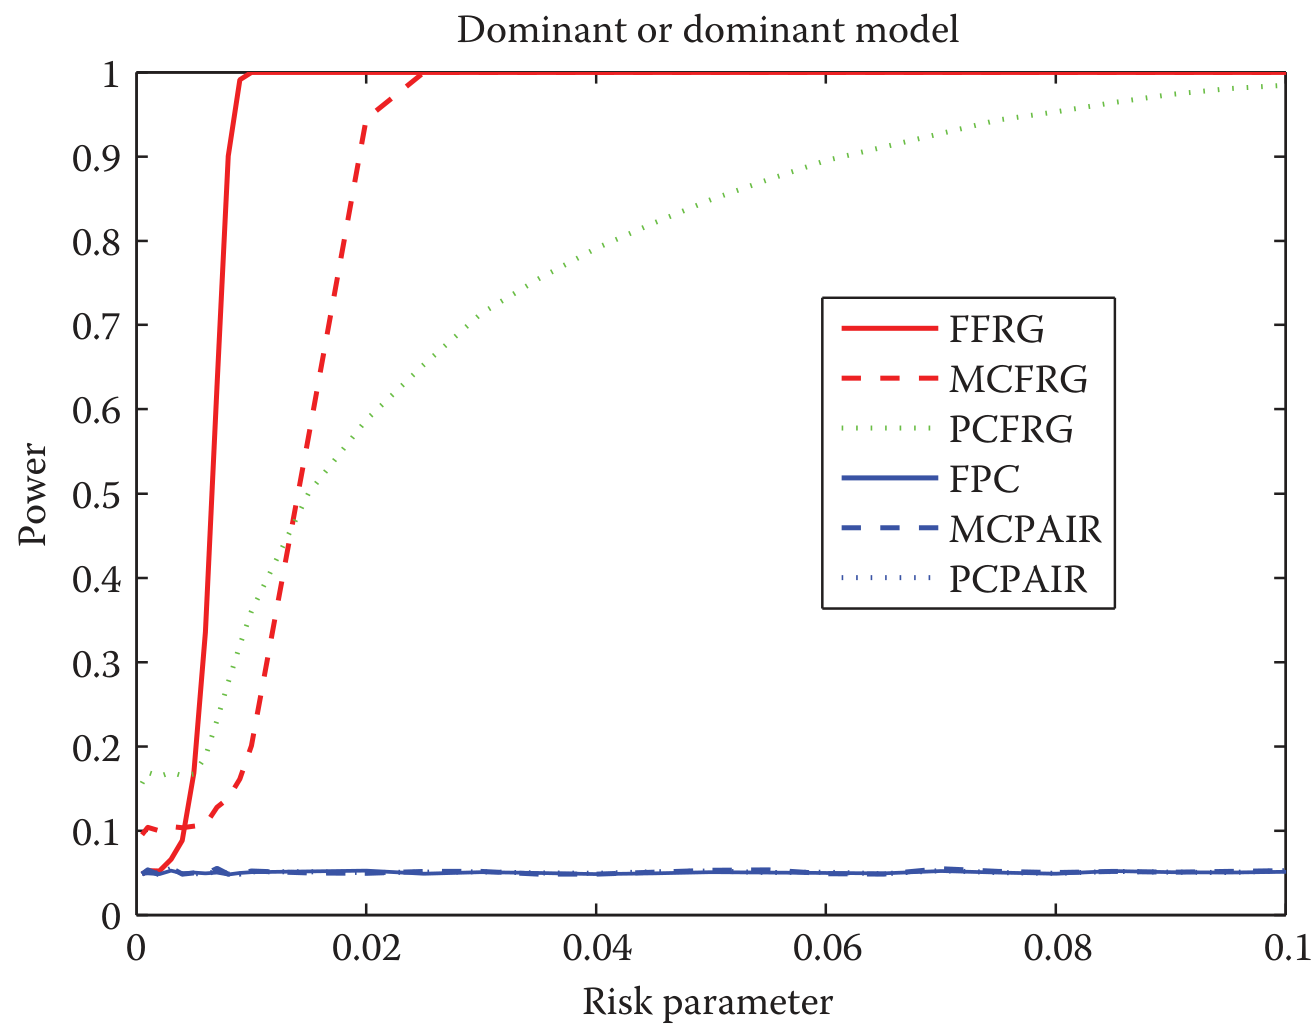
\includegraphics[width=13.8cm]{figures/ch03_fig23_data.png}};
\fill[white] (6.0740,0.0415) rectangle (8.7836,0.5138);
\node[font=\small,rotate=0,inner sep=0] at (7.4288,0.2776) {风险参数};
\fill[white] (0.1256,5.0373) rectangle (0.6084,6.1972);
\node[font=\small,rotate=90,inner sep=0] at (0.3670,5.6172) {统计功效};
\fill[white] (4.7583,10.2349) rectangle (10.0994,10.7071);
\node[font=\small,rotate=0,inner sep=0] at (7.4289,10.4710) {显性或显性模型};
\end{tikzpicture}
\origfig{23}{显性或显性模型下六种统计量 F-FRG、MC-FRG、PC-FRG、FPC-FPC、PC-pair-wise 和 MC-pair-wise 的功效曲线。}
\label{fig:ch03-23}
\end{figure}

\begin{figure}[htbp]
\centering
\begin{tikzpicture}[x=1cm,y=1cm]
\node[anchor=south west,inner sep=0] at (0,0) {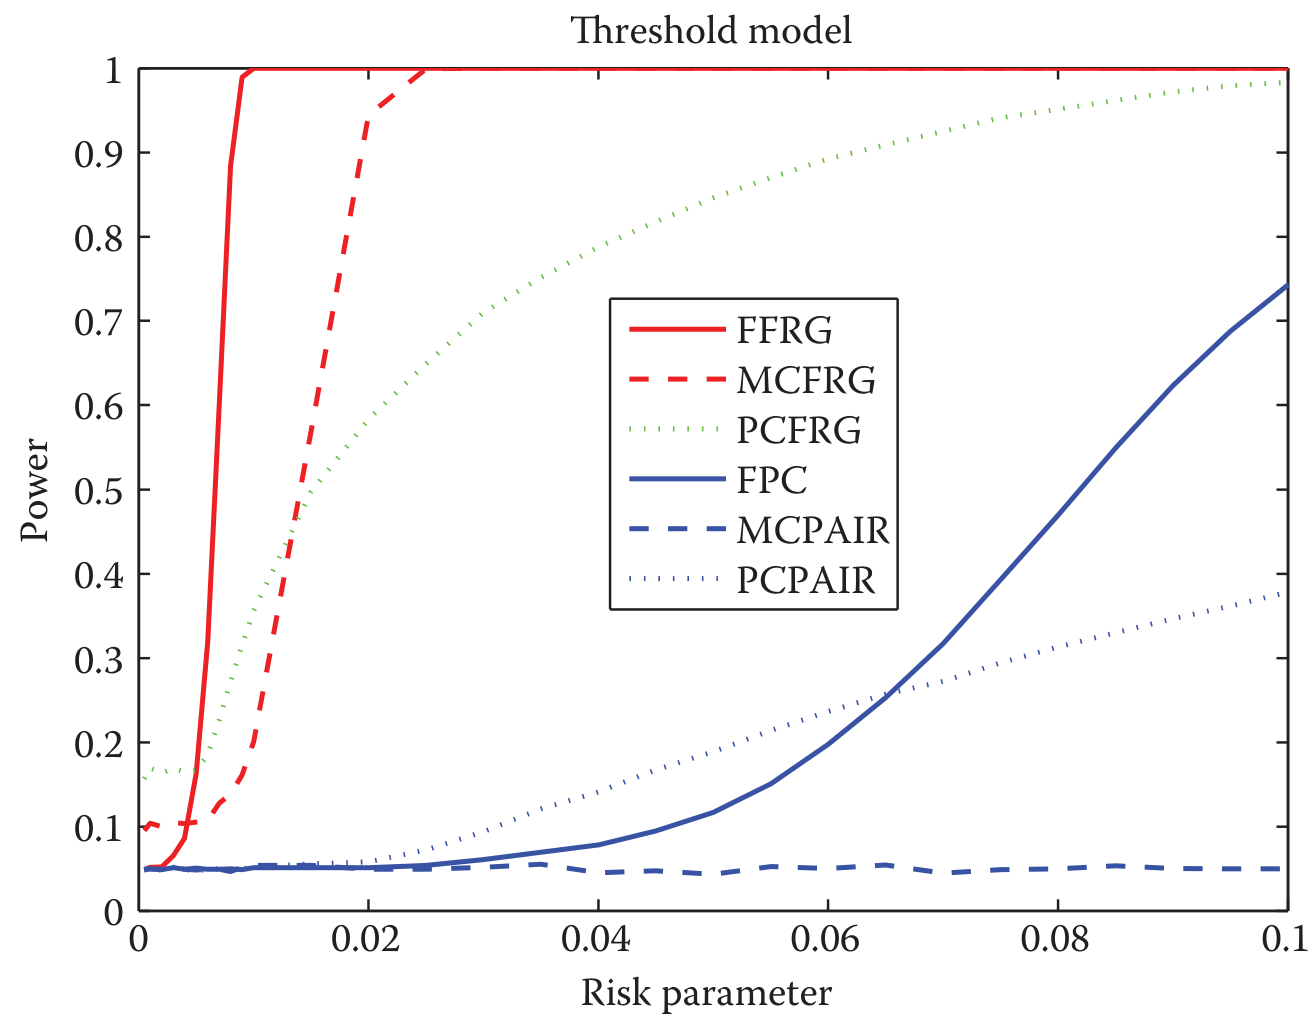
\includegraphics[width=13.8cm]{figures/ch03_fig24_data.png}};
\fill[white] (6.0626,0.0321) rectangle (8.7723,0.5043);
\node[font=\small,rotate=0,inner sep=0] at (7.4174,0.2682) {风险参数};
\fill[white] (0.1494,4.9754) rectangle (0.6321,6.1352);
\node[font=\small,rotate=90,inner sep=0] at (0.3908,5.5553) {统计功效};
\fill[white] (5.9450,10.1204) rectangle (8.9766,10.5927);
\node[font=\small,rotate=0,inner sep=0] at (7.4608,10.3566) {阈值模型};
\end{tikzpicture}
\origfig{24}{阈值模型下六种统计量 F-FRG、MC-FRG、PC-FRG、FPC-FPC、PC-pair-wise 和 MC-pair-wise 的功效曲线。}
\label{fig:ch03-24}
\end{figure}


这些曲线给出显著性水平 $\alpha=0.05$ 下，功效随风险参数的变化。从图中可见几个显著特点。第一，在全部四种交互作用模型下，基于 FRG 的检验功效最高。F-FRG 利用了将表型和基因型均视为函数的优势，把随时间变化的表型函数分解为时间的正交特征函数，把随位置变化的基因型函数分解为基因组位置的正交特征函数。F-FRG 同时降低表型变异和基因型变异的维数，仅用少数特征函数表示变异，从而提高检验的统计功效。

第二，F-FRG 与其余五种模型的功效差异很大。第三，数据包括性状值和基因型值，两者均可采用三类取值：函数（曲线）值、均值和逐点值（时间点或基因组位置）。当基因型采用函数值时，检验功效由高到低依次为 F-FRG、MCFRG 和 PCFRG；若考虑每个 SNP 的基因型值，PC-pair-wise 检验的功效则高于 MC-pair-wise 检验。第四，传统均值横断面两两检验（MCPAIR）的功效远低于 F-FRG。在许多情形下，MCPAIR 无法检出两个基因之间的交互作用。
\FloatBarrier

\subsection{真实数据分析}

为进一步评价性能，将 F-FRG 应用于得克萨斯州斯塔尔县的血氧饱和度研究。血氧饱和度信号按秒测量，一夜共获得35,280次测量。血氧饱和度可为阻塞性睡眠呼吸暂停患者的睡眠质量提供重要信息（Nieto et al. 2000）。对来自斯塔尔县的833名墨西哥裔美国人，在20,763个基因中共分型406,299个 SNP。F-FRG 需要将基因型函数按特征函数展开，每个基因至少需要3个 SNP，因此排除仅含1个或2个 SNP 的基因。最终分析17,258个基因，共有148,910,653对不同基因。采用 Bonferroni 方法校正多重检验后，判定显著性的 $P$ 值阈值为 $3.36\times10^{-10}$。为减少纳入分析的测量次数，以每10秒血氧饱和度的均值作为性状值，并将基因两侧5 kb 区域内的 SNP 视为属于该基因。为保证数值稳定性，使用奇异值分解计算矩阵的逆，保留能解释总变异99\%的奇异值数量。

共发现13对具有显著交互作用的基因，涉及23个基因，$P$ 值介于 $2.27\times10^{-10}$ 与 $4.85\times10^{-43}$ 之间（表3.8）。除以完整的血氧饱和度曲线作为函数型响应外，还将其均值作为标量响应变量，采用 MC-FRG 检验交互作用。表3.8还给出以性状瞬时值作为表型、用简单回归交互作用模型检验两个基因间全部可能 SNP 对的交互作用时，在全部观测时段上的最小 $P$ 值；每个 SNP 对的两个 SNP 分别位于不同基因。

\begin{table}[htbp]
\centering
\origtable{8}{FRG 识别的13对具有显著交互作用基因的 $P$ 值。}
\label{tab:ch03-08}
\small
\setlength{\tabcolsep}{4pt}
\begin{tabular}{rlrlrrrr}
\toprule
\multirow{2}{*}{染色体} & \multirow{2}{*}{基因1} & \multirow{2}{*}{染色体} & \multirow{2}{*}{基因2} & \multirow{2}{*}{配对数} & \multicolumn{3}{c}{$P$ 值}\\
\cmidrule(lr){6-8}
&&&&&F-FRG&\shortstack{横断面\\FRM}&\shortstack{SRG\\（最小值）}\\
\midrule
9 & MIR4520A & 9 & MIR4520B & 9 & 4.85E-43 & 3.92E-36 & 0.00469\\
1 & DPH2 & 1 & ATP6V0B & 9 & 2.55E-37 & 2.86E-31 & 5.93E-05\\
22 & MAK16 & 22 & TTI2 & 25 & 7.59E-33 & 1.86E-21 & 0.01894\\
4 & TAS2R5 & 4 & TAS2R31 & 32 & 2.99E-27 & 2.01E-25 & 0.03168\\
16 & FAM211B & 16 & GGT1 & 12 & 4.42E-23 & 2.09E-11 & 0.01246\\
17 & OR5H15 & 17 & OR5H14 & 25 & 4.47E-17 & 3.92E-07 & 0.00042\\
22 & MIR378D2 & 22 & PDP1 & 9 & 3.10E-14 & 1.28E-07 & 0.00896\\
9 & MIR4520A & 9 & C17orf100 & 12 & 6.41E-14 & 9.95E-02 & 0.00020\\
9 & MIR4520B & 9 & C17orf100 & 12 & 6.41E-14 & 9.95E-02 & 0.00020\\
8 & WDR90 & 8 & RHOT2 & 9 & 2.43E-13 & 1.57E-04 & 0.00022\\
11 & B9D2 & 11 & TMEM91 & 18 & 1.15E-11 & 5.38E-08 & 7.76E-14\\
8 & KCTD1 & 8 & TAOK2 & 20 & 9.52E-11 & 6.74E-04 & 0.00550\\
21 & MIR489 & 21 & MIR653 & 9 & 2.27E-10 & 1.10E-02 & 0.00691\\
\bottomrule
\end{tabular}
\end{table}


可以看到，F-FRG 交互作用检验的 $P$ 值远小于逐点两两检验（MC-FRG）。F-FRG 利用将表型与基因型均视为函数的优势，把随时间变化的表型函数分解为时间的正交特征函数，把随位置变化的基因型函数分解为基因组位置的正交特征函数。只使用能够捕捉性状函数与基因型函数主要信息的少数特征函数，表示性状变异与遗传变异。这使数据的表型变异和基因型变异两个方面的维数均大幅降低。
\FloatBarrier
